\chapter{Project Execution, Monitoring and Control}
\label{chap:pe}
\section{Project Status: Friday Week 9}
\label{sec:ps1}
We finished all the features required in the initial development process on May 18, 2020. However, because the document has to be updated to version 1.1 before May 23, 2020, we can’t update artefacts generated by the second sprint review meeting and the second sprint retrospective to the document in this version. And we would decide whether the third sprint is needed in the comming sprint review. The online store can now be accessed on \textit{https://pinwang4.wixsite.com/website}. It is a beautiful and well designed site, with a user-friendly interface and all the features required in the initial development. A screenshot of the homepage is available in Figure \ref{fig:homepage}

We use a handy tool called \textit{Trello}\footnote{To join the Agile Board: https://trello.com/invite/b/ZqSHe7MR/9b942f7a393fb08379c206fb2064726a/spm-group-project} to manage our Agile Board. The feature cards in the Agile Board are set by the Scrum Master with tasks checklist defined inside them. Students in the development team would add themselves to a specific card and move the card to the \textit{TODO} list after the Daily Scrum standup meeting. A card is moved to \textit{DONE} list only if all the tasks in it are finished and pass tests. The total finish story points can be quickly check in the upper left corner of the \textit{DONE} list. By checking the card in the \textit{DONE} list, the Scrum Master can keep track of everyone’s contribution. A screenshot of the Agile Board system is shown in Figure 4.4.

The burndown chart is updated by the Scrum Master after every daily standup. By comparing the actual jagged line with the ideal schedule straight line, the Scrum Master can easily evaluate whether the development team is working efficiently, whether the sprint backlog can be finished on time and whether the progress of the project is hindered. Also, the burndown chart is used to re-estimate the velocity of the development team. 

In the first sprint, we held daily scrum standup meeting every workday. But since in the first sprint retrospective, our development team said that they might not work for this subject every day and the Daily Scrum Meeting is held too often. So we change the process to be held only on Monday, Wednesday and Friday. The daily scrum meetings are thought to be very useful since it not only can help our development team to improve their work efficiency but also let other knows what they are working on and what should be solved on a specific date. As mention in Section \ref{sec:constraints}, our team is facing some time difference problem. Daily Scrum were conducted via chat. We do it in the daily-scrum channel in \textit{Slack}. An example of how our daily scrum standup meeting system work is shown in Figure \ref{fig:dailyScrum} in Appendix B. The meeting record is shown in Table \ref{tab:dailyScrumStandupMeetingRecord} in Appendix B.

At the end of the first sprint, a sprint review is held to give a demo on the product to determine what are finished and what are not. The demo is excellent, and together we find out that some unworkable buttons should be deleted in the delivery version. After the sprint review, a sprint retrospective was held to help improve the team's efficiency. All the members in the development team thought the Daily Scrum is great. However, it is held too often since they have to learn other subjects. So, we decide to hold daily scrum standup only on Monday, Wednesday and Friday in the second sprint. The Record of the first pprint review and sprint retrospective can be found in \textit{https://www.youtube.com/watch?v=4slzV0LbUSY}.

\subsection{Process Related Artefacts}  
The Meeting Minutes can be found in Appendix A and the Daily Scrum Standup Meeting Record can be found in Appendix B. 

\textbf{Burndown Chart for the Whole Project}

\begin{figure}[htp]
\centering
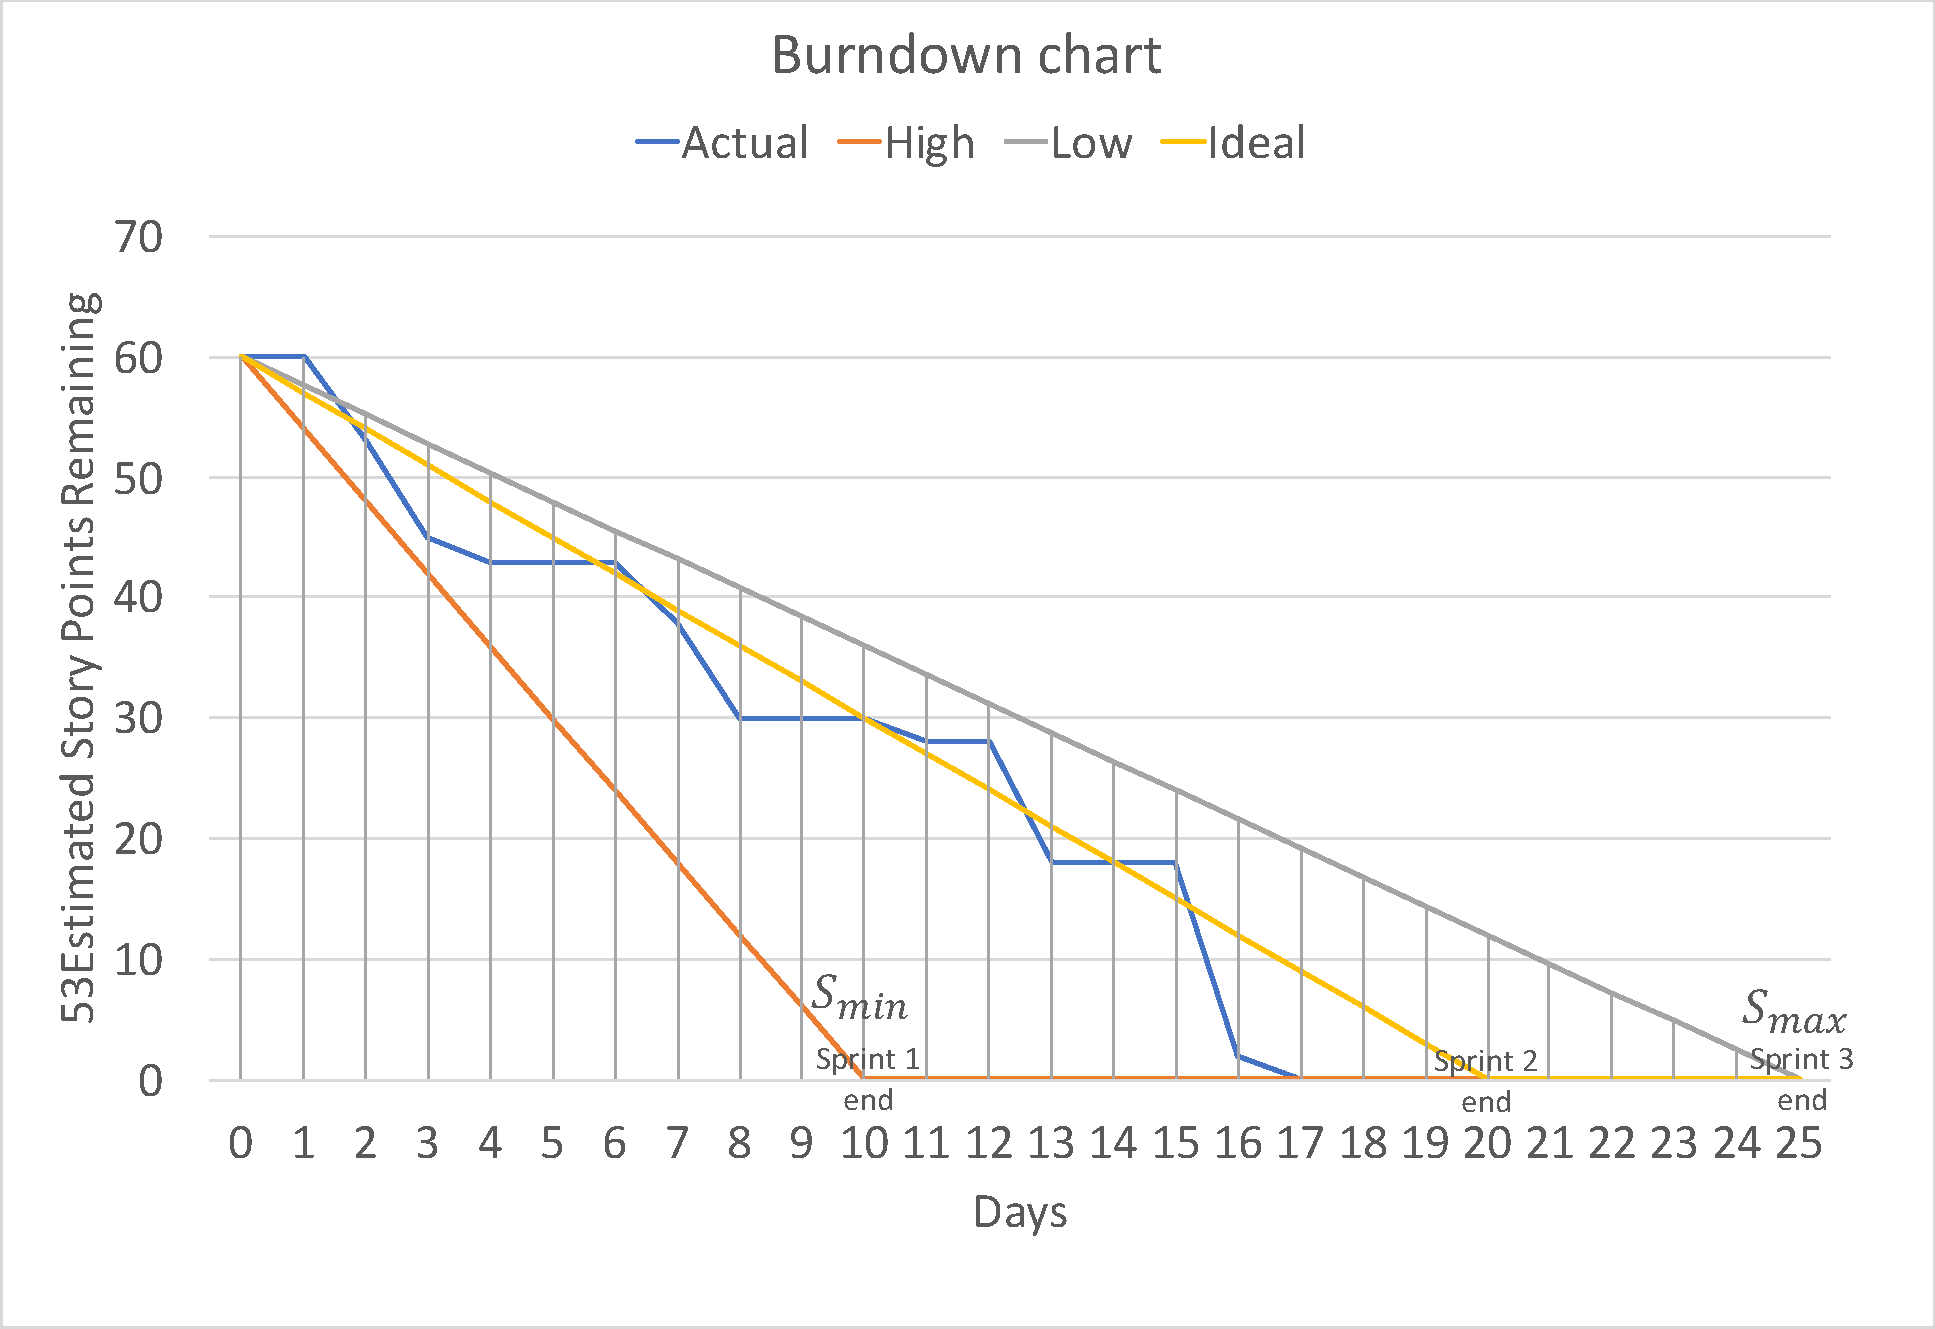
\includegraphics[width=\textwidth]{Figures/totalBurndown.pdf}
\caption{Burndown Chart of the Whole Project}
\label{fig:totalBurndown}
\end{figure}

\clearpage
\textbf{Burndown Chart for the First Sprint (April, 27 - May, 8)}
\begin{figure}[htp]
\centering
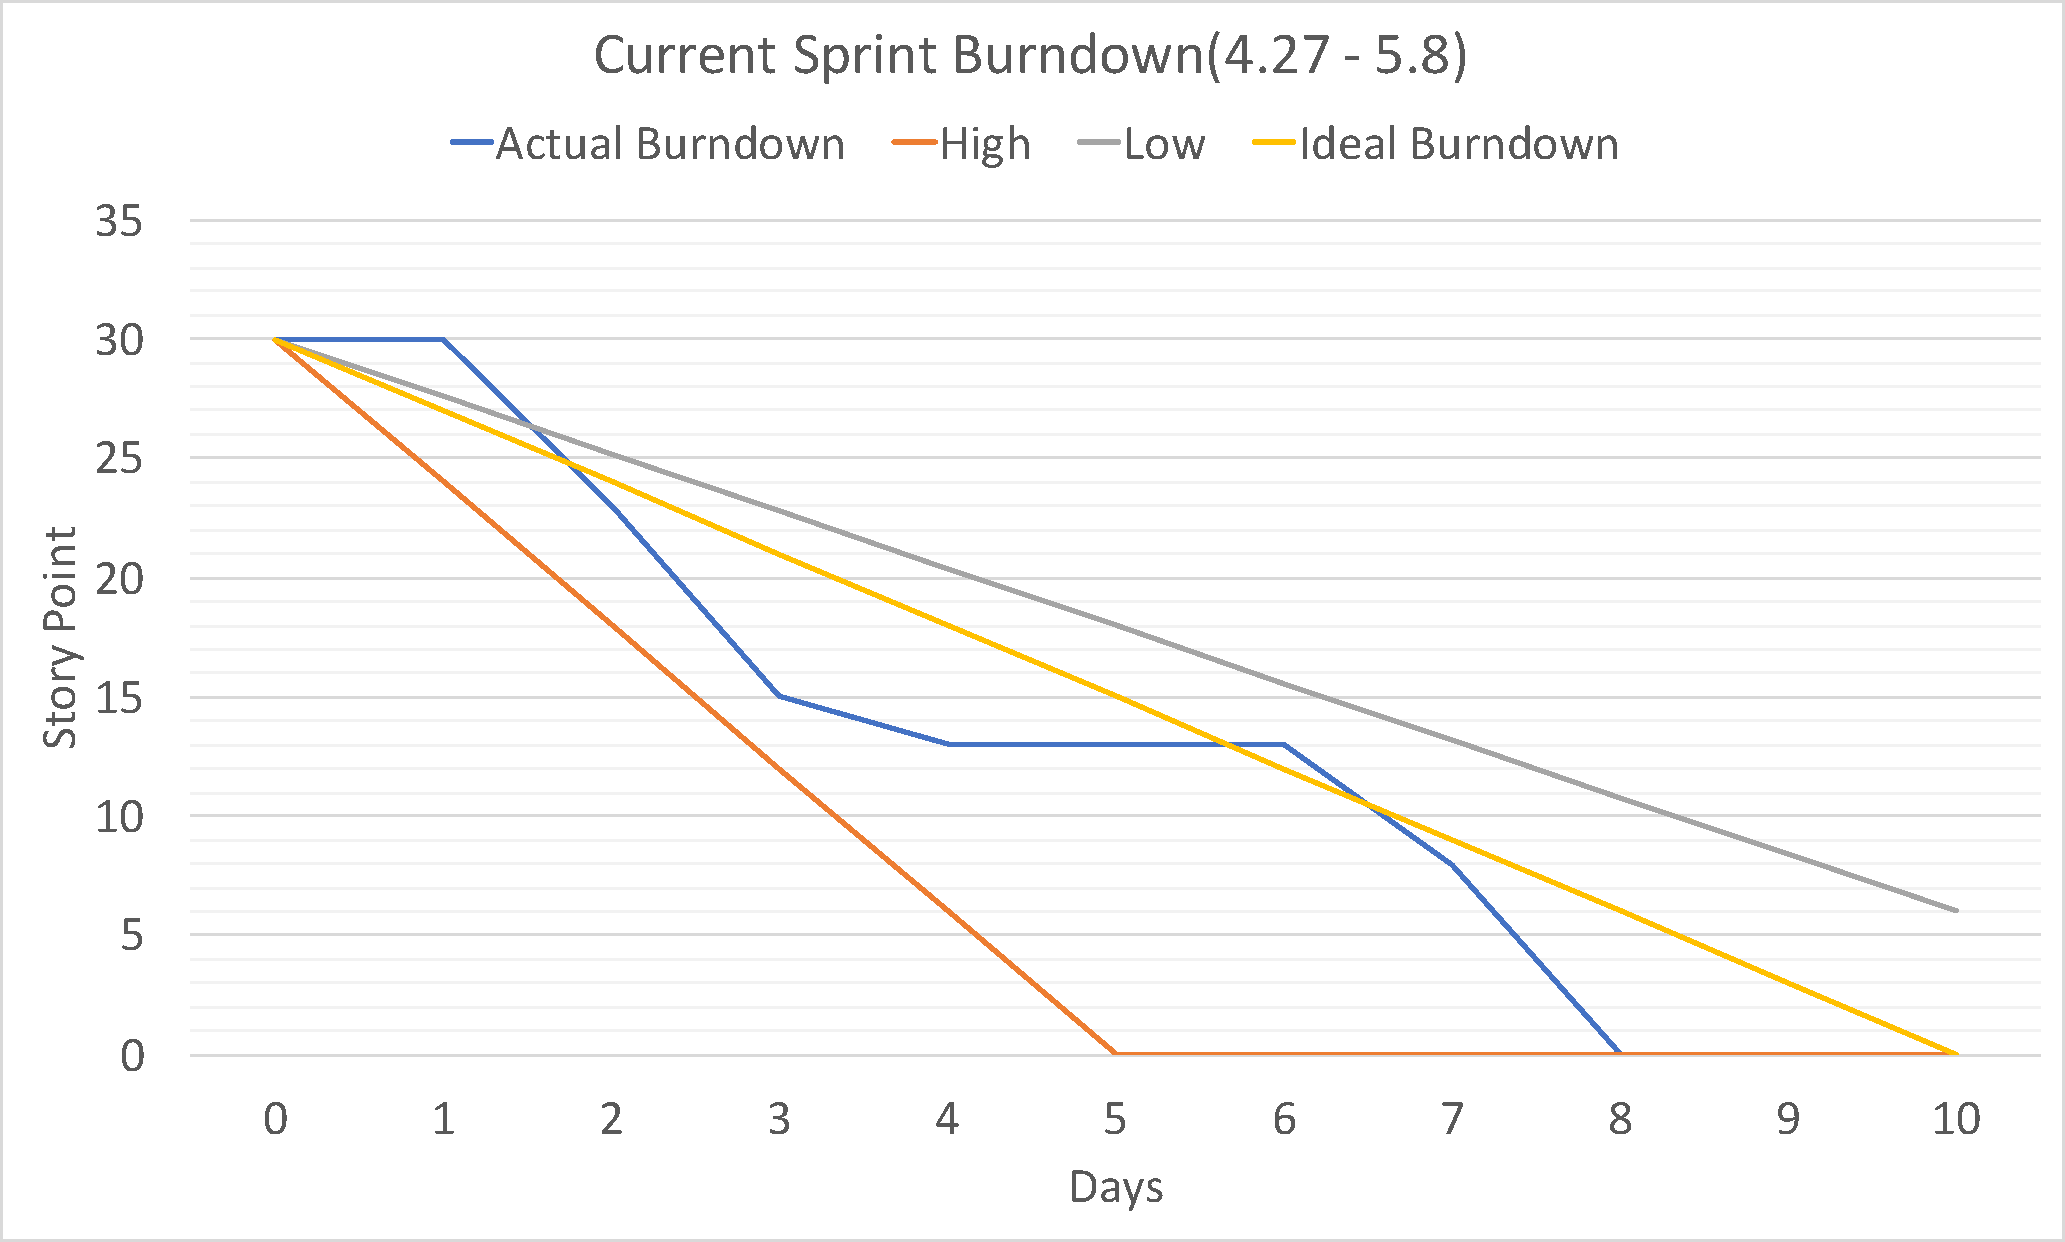
\includegraphics[width=0.65\textwidth]{Figures/sprint1Burndown.pdf}
\caption{Burndown Chart of the First Sprint}
\label{fig:sprint1Burndown}
\end{figure}
\\
\textbf{Burndown Chart for the Second Sprint (May, 11 - May, 22)}
\begin{figure}[htp]
\centering
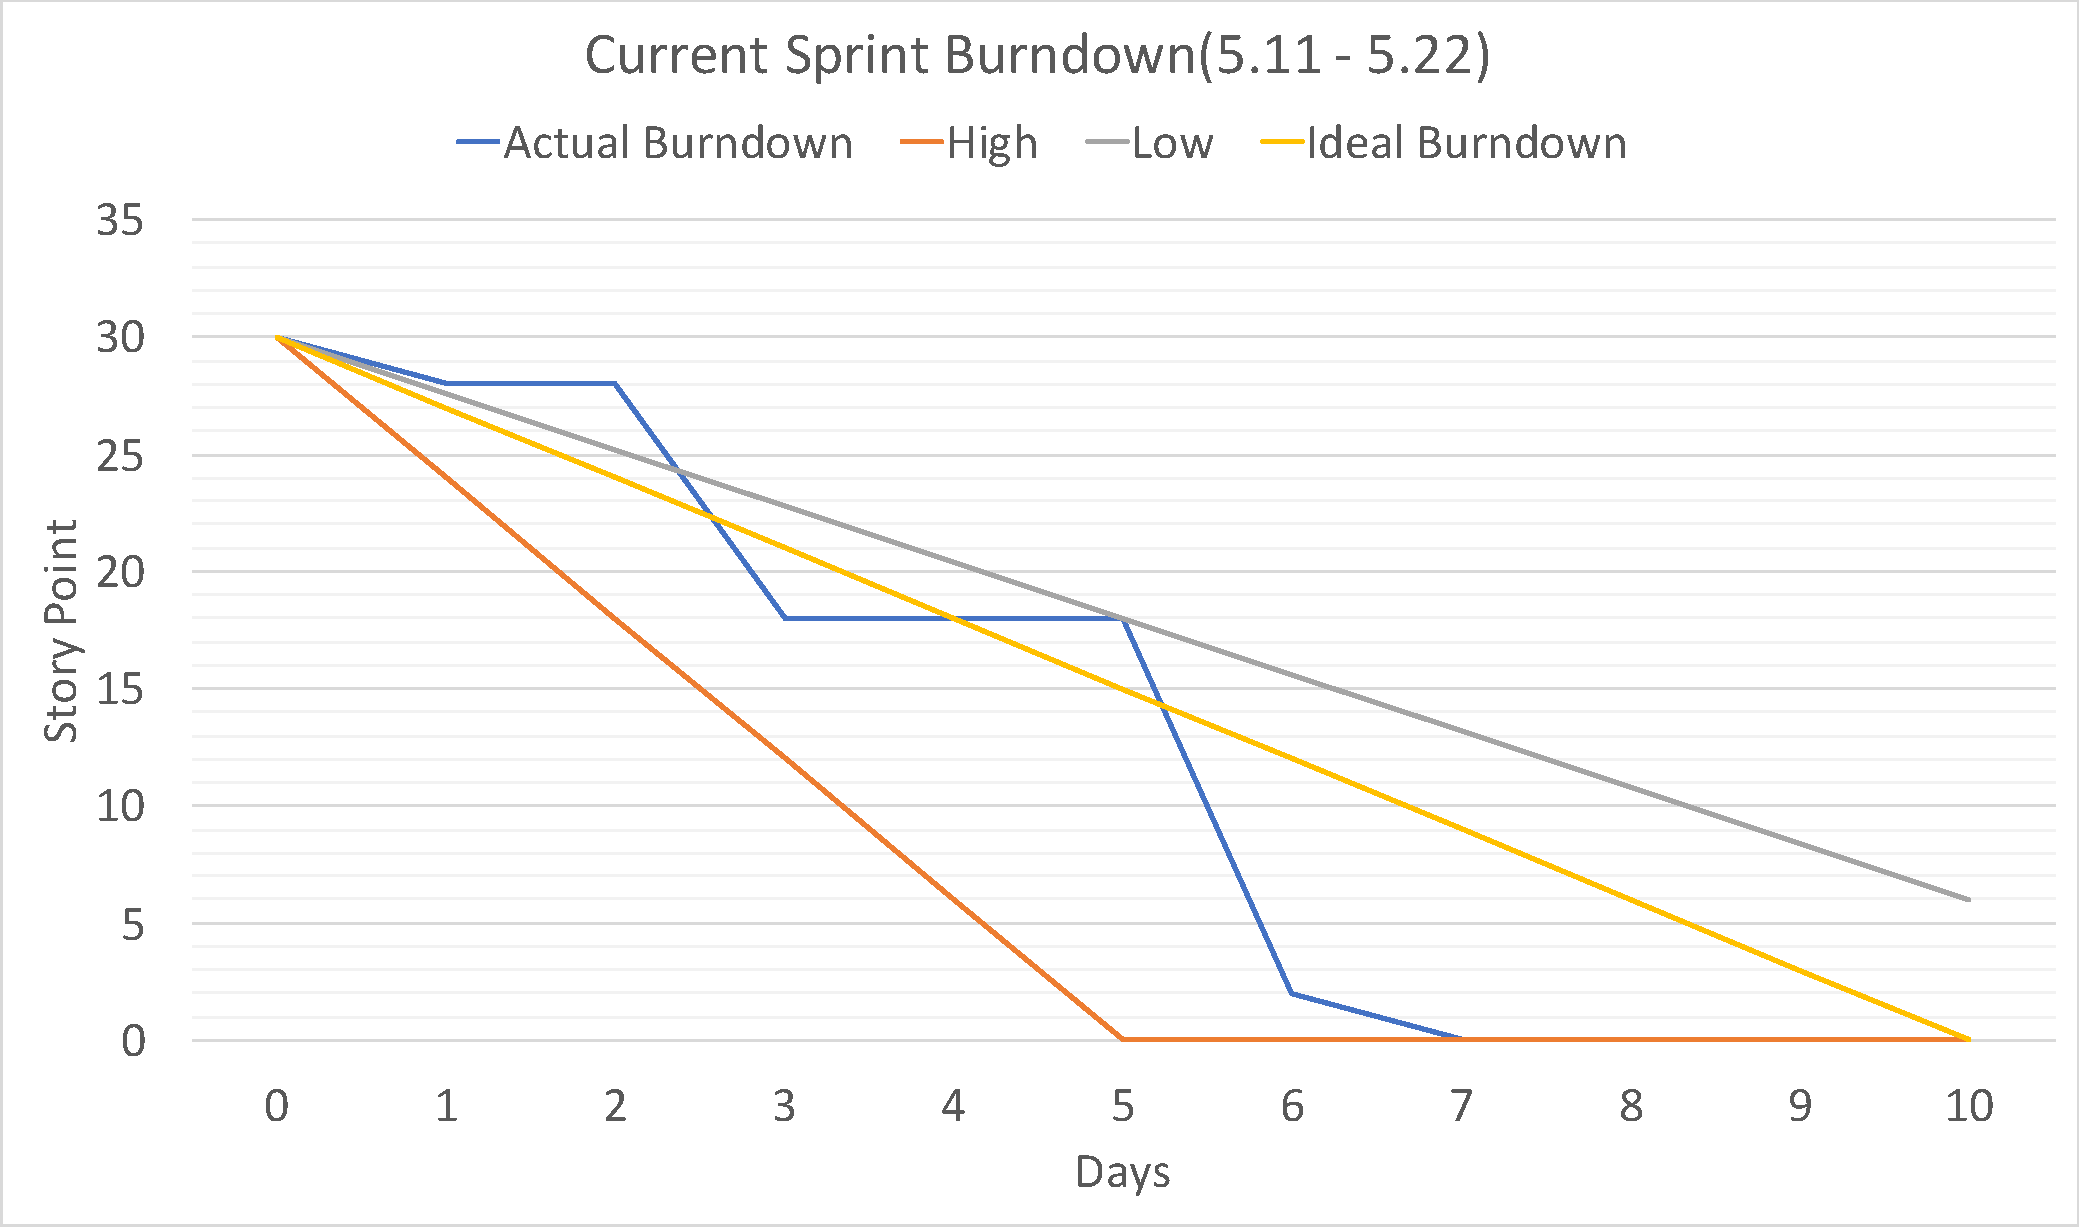
\includegraphics[width=0.65\textwidth]{Figures/sprint2Burndown.pdf}
\caption{Burndown Chart of the Second Sprint}
\label{fig:sprint2Burndown}
\end{figure}

\clearpage
\textbf{Agile Board}
\\
A handy tool called \textit{Trello} is used to manage our Agile Board. As present, all basic features have been realized. The Agile Board system is shown in Figure \ref{fig:agileBoard}:

\begin{figure}[htp]
\centering
\includegraphics[width=\textwidth]{Figures/agileBoard.png}
\caption{Agile Board}
\label{fig:agileBoard}
\end{figure}

%%%%%%%%%%%%%%%%%%%%%% Agenda %%%%%%%%%%%%%%%%%%%%%%%%%%%%%%%%
\clearpage
\textbf{Agenda}
\begin{tabularx}{0.95\linewidth}{%
  >{\raggedright\arraybackslash}p{0.15\linewidth}%
  >{\raggedright\arraybackslash}p{0.18\linewidth}%
  >{\raggedright\arraybackslash}p{0.12\linewidth}%
  >{\raggedright\arraybackslash}p{0.5\linewidth}
  }
  \toprule
  Date & Attendees & Format & Topic
  \\
  \midrule
  10 pm, April 12, 2020
  & Yicun Tian,\newline Hongkang Li,\newline Pin Wang,\newline Chongjing Zhang,\newline Zhangfeng Qiu
  & Virtual Meeting – Zoom
  & 
  1. Team creation and bonding.\newline
  2. Tasks Assignment.
  \\
  %%%%%%%%%%%%%%%%%%%%%%%%%%%%%%%%%%%%%%%%%%%%%%%%%%%
  \\
  \midrule
  5 pm, April 15, 2020
  & Yicun Tian,\newline Pin Wang,\newline Zhangfeng Qiu
  & Virtual Meeting – Zoom
  & 
  1. Initial project manage planing document job assignment.
  \\
  %%%%%%%%%%%%%%%%%%%%%%%%%%%%%%%%%%%%%%%%%%%%%%%%%%%
  \midrule
  5 pm, April 17, 2020
  & Yicun Tian,\newline Hongkang Li,\newline Pin Wang,\newline Chongjing Zhang,\newline Zhangfeng Qiu
  & Virtual Meeting – Zoom
  & 
  1. Requirement Breakdown.\newline
  2. User Story definition.\newline
  3. Product backlog definition.\newline
  4. User point and value point estimation.\newline
  5. Feature tasks break down.
  \\
  %%%%%%%%%%%%%%%%%%%%%%%%%%%%%%%%%%%%%%%%%%%%%%%%%%%
  \midrule
  3 pm, April 26, 2020
  & Yicun Tian,\newline Hongkang Li,\newline Pin Wang,\newline Chongjing Zhang,\newline Zhangfeng Qiu
  & Virtual Meeting – Zoom
  & 
  1. Discuss risks of the project.\newline
  2. Discuss stake holders of the project.\newline
  3. Decide the process we would go through in our first Sprint.\newline
  4. First Sprint Planning.
  \\
  %%%%%%%%%%%%%%%%%%%%%%%%%%%%%%%%%%%%%%%%%%%%%%%%%%%
  \midrule
  6 pm, April 28, 2020
  & Yicun Tian,\newline Zhangfeng Qiu
  & Virtual Meeting – Zoom
  & 
  1. Meeting with Subject Matter Experte -- Rajesh Chittor
  \\
  %%%%%%%%%%%%%%%%%%%%%%%%%%%%%%%%%%%%%%%%%%%%%%%%%%%
  \midrule
  3 pm, May 9, 2020
  & Yicun Tian,\newline Hongkang Li,\newline Pin Wang,\newline Chongjing Zhang,\newline Zhangfeng Qiu
  & Virtual Meeting – Zoom
  & 
  1. SPRINT REVIEW \newline 
  2. SPRINT RETROSPECTIVE
  \\
  %%%%%%%%%%%%%%%%%%%%%%%%%%%%%%%%%%%%%%%%%%%%%%%%%%%
  \midrule
  3 pm, May 24, 2020
  & Yicun Tian,\newline Hongkang Li,\newline Pin Wang,\newline Chongjing Zhang,\newline Zhangfeng Qiu
  & Virtual Meeting – Zoom
  & 
  1. SPRINT REVIEW \newline 
  2. SPRINT RETROSPECTIVE
  \\
  %%%%%%%%%%%%%%%%%%%%%%%%%%%%%%%%%%%%%%%%%%%%%%%%%%%
  \midrule
  15-minute every workday (April, 27 - May, 8)
  & Yicun Tian,\newline Hongkang Li,\newline Pin Wang,\newline Chongjing Zhang,\newline Zhangfeng Qiu
  & Casual Chat on Slack
  & 
  The first sprint Daily Scrum Standup:
  \begin{enumerate}
    \item What the development team did yesterday.
    \item What the development team plan to do today.
    \item Block on the way.
  \end{enumerate}
  \\
  %%%%%%%%%%%%%%%%%%%%%%%%%%%%%%%%%%%%%%%%%%%%%%%%%%%
  \midrule
  15-minute, on Monday, Wednesday, Friday (May, 11 - May, 22)
  & Yicun Tian,\newline Hongkang Li,\newline Pin Wang,\newline Chongjing Zhang,\newline Zhangfeng Qiu
  & Casual Chat on Slack
  & 
  The second sprint Daily Scrum Standup
  \begin{enumerate}
    \item What the development team did in the last two day.
    \item What the development team plan to do today and tomorrow.
    \item Block on the way.
  \end{enumerate}
  \\
  \bottomrule
  \\
  \caption{Agenda}  
  \label{tab:agenda}
\end{tabularx}
%%%%%%%%%%%%%%%%%%%%%%%%%%%%%%%%%%%%%%%%%%%%%%%%%%%%%%

\textbf{The First Sprint Review \& Sprint Retrospective Record (May, 8, 2020)}
\\
The record of these two meetings can be found on \textit{https://www.youtube.com/watch?v=4slzV0LbUSY}.

In the sprint review, the development team give a presentation to show all the features finished in the first sprint. The Scrum Master and the Product Owners provide reviews for the product. We held the meeting in zoom. From the demo, we find out that there are some unworkable buttons which should be deleted in the delivery version. And after a little change based on the reviews, we release our first product to the market.

In the sprint retrospective, we discuss what went well in the first sprint. All the member in the development team thinks Daily Scrum is great. It helps the development team communicate better because it can provide information about what others are doing. When it comes to the "what could be improved" part, we decide to hold daily scrum standup only on Monday, Wednesday and Friday. This is because the development team would not work on this subject every day.

\subsection{Product Related Artefacts}
\textbf{The status of the product}
\\
We have finished all the features required in the initial development process. The online store website can be accessed now on \textit{https://pinwang4.wixsite.com/website}. A screenshot of the homepage is shown in Figure \ref{fig:homepage}. The online store website is beautiful and well designed, with a user-friendly interface and all the features required in the initial development. The product design can be found in Appendix C. The use cases and user stories of the product is shown in Table \ref{tab:productBacklog} in Section \ref{sec:productBacklog}, which would not be shown again here. The detail of the features completed in each sprint can be checked in Section \ref{sec:sprintCycle}. Also the completed features detail can be check in our Agile Board in \textit{Trello}, which is shown in Figure \ref{fig:doneFeature}. For a quick look, a completed feature lists (detailed tasks breakdown would not be included here) is provided below:
\\
\begin{itemize}
  \item Milestone 1 -- let the website go online without the function of purchase. The website can display all kinds of information about the products and provide the service of user registration. At the same time, the database is initially established to record the data of users and products.
  \begin{enumerate}
    \item Datebase
    \item Browse product menu
    \item Customer sign up
    \item Customer sign in and sign out
    \item Customer add and edit client information
    \item Admin manage product infomation
    \item Admin sign in and sign out
  \end{enumerate}
  \item Milestone 2 -- Allow users to place orders to purchase products. After this milestone, sellers can view and modify user orders. Basic requirement testing has to be passed in this milestone.
  \begin{enumerate}
    \item Customer add products to shopping cart
    \item Customer manage shopping cart
    \item Customer check out shopping cart
    \item Customer cancel orders
    \item Admin view and manage orders
    \item Register admin account
    \item Edit admin account information
  \end{enumerate}
\end{itemize}

\begin{figure}[htp]
\centering
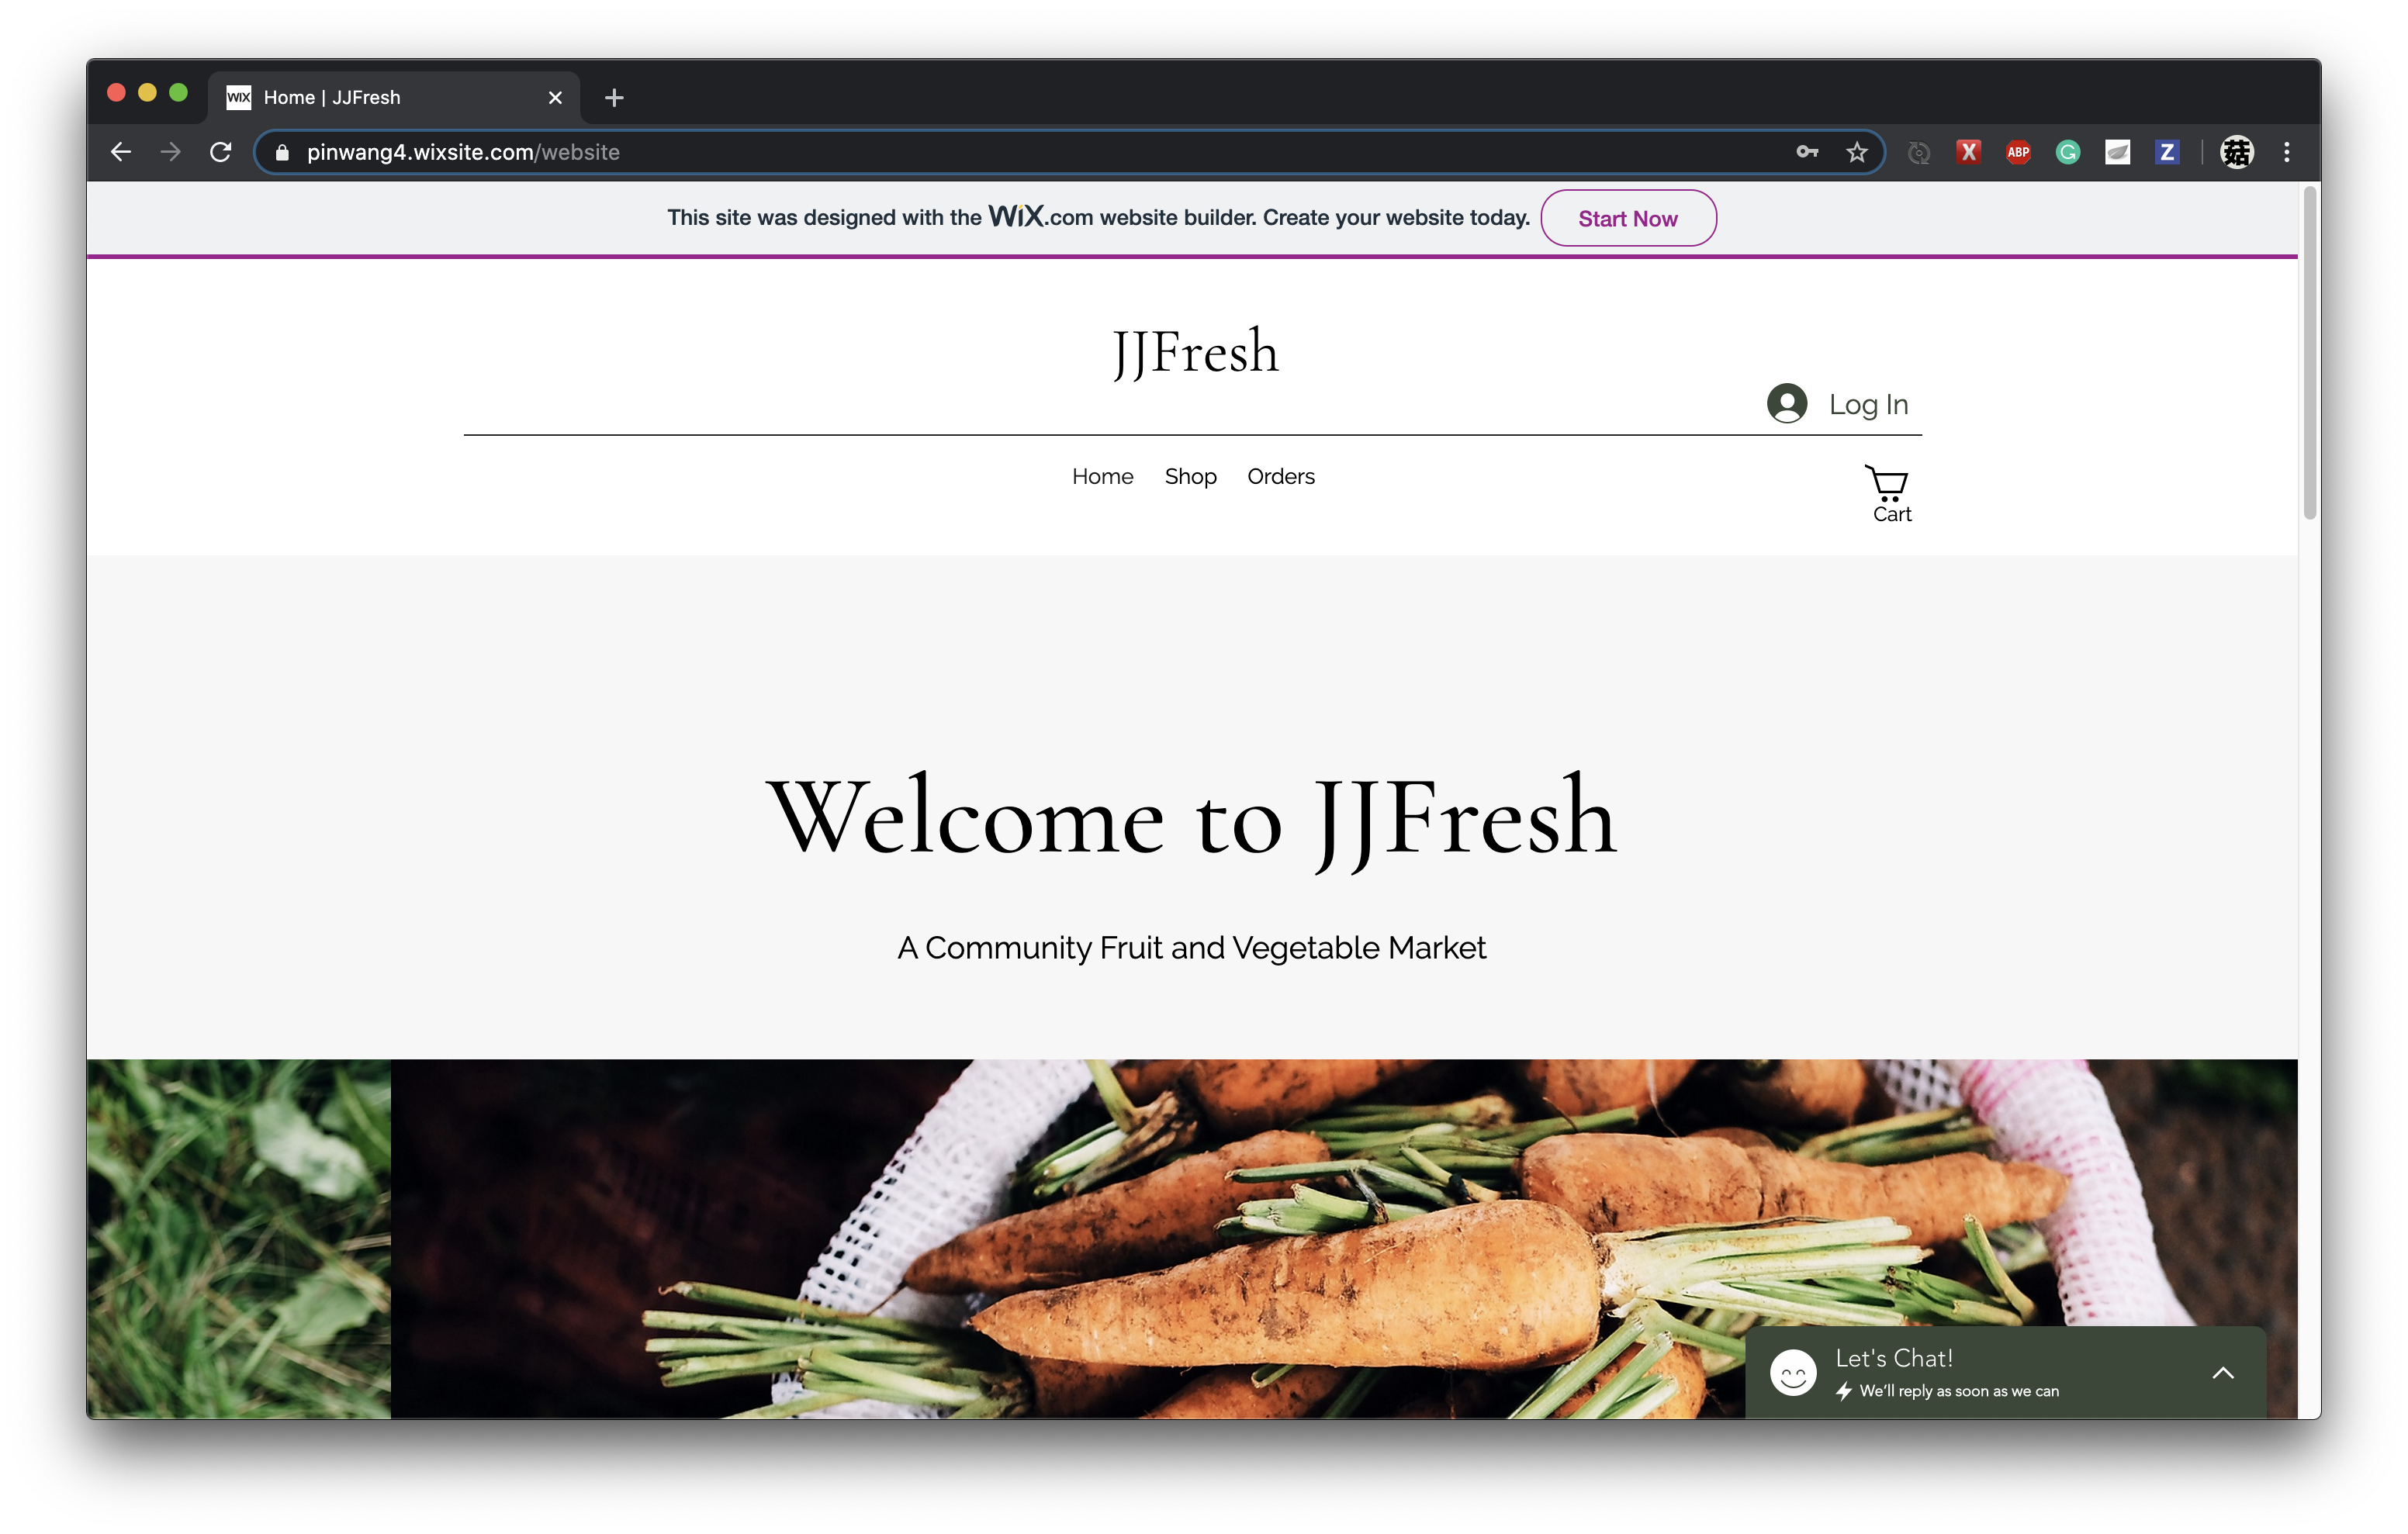
\includegraphics[width=\textwidth]{Figures/homepage.png}
\caption{Homepage of the online store}
\label{fig:homepage}
\end{figure}

\begin{figure}[htp]
\centering
\includegraphics[width=\textwidth]{Figures/doneFeature.png}
\caption{Done list in the Agile board}
\label{fig:doneFeature}
\end{figure}

\clearpage
\subsection{Risk Monitoring and Control}
\label{sub:riskMonitoringandControl}
So far, the project has completed all the basic functions, but the four risks defined in the initial stage of development have not yet occurred. One of the main reasons is that the product has not been used. In other words, the risks defined in Section \ref{sec:riskManagement} all occur after the product is put into use or after simulated use. Therefore, after the product owner, which is a member of our group, simulates the user for testing, we will further analyze these four risks.
At the same time, the development process was relatively smooth, and the plan was completed in advance. Therefore, we have not defined new risks at present.

%%%%%%%%%%%%%%%%%%%%%%%%%%%%%%%%%%%%%%%%%%%%%%%%%%%%%%%%%%%%%%%%%%%%%%%%%%%%%%%%

\section{Project Status: Friday week 10}
\label{sec:ps2}
Because all the basic features have been implemented in the last status, not much update will be provided in this version. In the second Sprint view, we found out some bugs together. The address and the email of the customers cannot show correctly in the order management page of the administer. But the development team fix the problems immediately, which didn't affect the delivery of the product. We finish the project in four weeks as expect. After discussion with the product owners, since all the application features work well and our development team becomes busy at the end of the semester, we decide to cancel the third sprint. Here we will provide some more details about our project and product.

%%%%%%%%%%%%%%%%%%%%%%%%%%%%%%%%%%%%%%%%%%%%%%%%%%%%%%%%%%%%%%%%%%%%%%%%%%%%%%%%

\subsection{Process Related Artefacts}
The Second Review \& Sprint Retrospective Record(Mar, 24, 2020)
The record of the Second Review \& Sprint Retrospective can be found on https://www.youtube.com/watch?v=KeiiwPMA5dU\&t=525s. 

In the second sprint review, the development gave a presentation to show all the features finished in the second sprint. The Scrum Master and the Product Owners provide a review of the product. We held the meeting in zoom. From the demo, we found out that the addresses and the emails of customers cannot show correctly in the order management page of the administer. The development team fixed the problems immediately. The new version of the product was delivered on time. We reach the second milestone successfully.

In the sprint retrospective, we discussed what went well in the first sprint. Half of the development team thought that it is better to do Daily Sprint Standup every day because, in this way, they feel more comfortable to come up with what to do and what they have done. And because the development team said that they are busy at the end of the semester and all the features have been finished well, they didn't want to have one more sprint. So, after discussion, we canceled the third sprint.

%%%%%%%%%%%%%%%%%%%%%%%%%%%%%%%%%%%%%%%%%%%%%%%%%%%%%%%%%%%%%%%%%%%%%%%%%%%%%%%%
\clearpage
\subsection{Product Related Artefacts}
\textbf{Use Case Diagram}
\begin{figure}[htp]
\centering
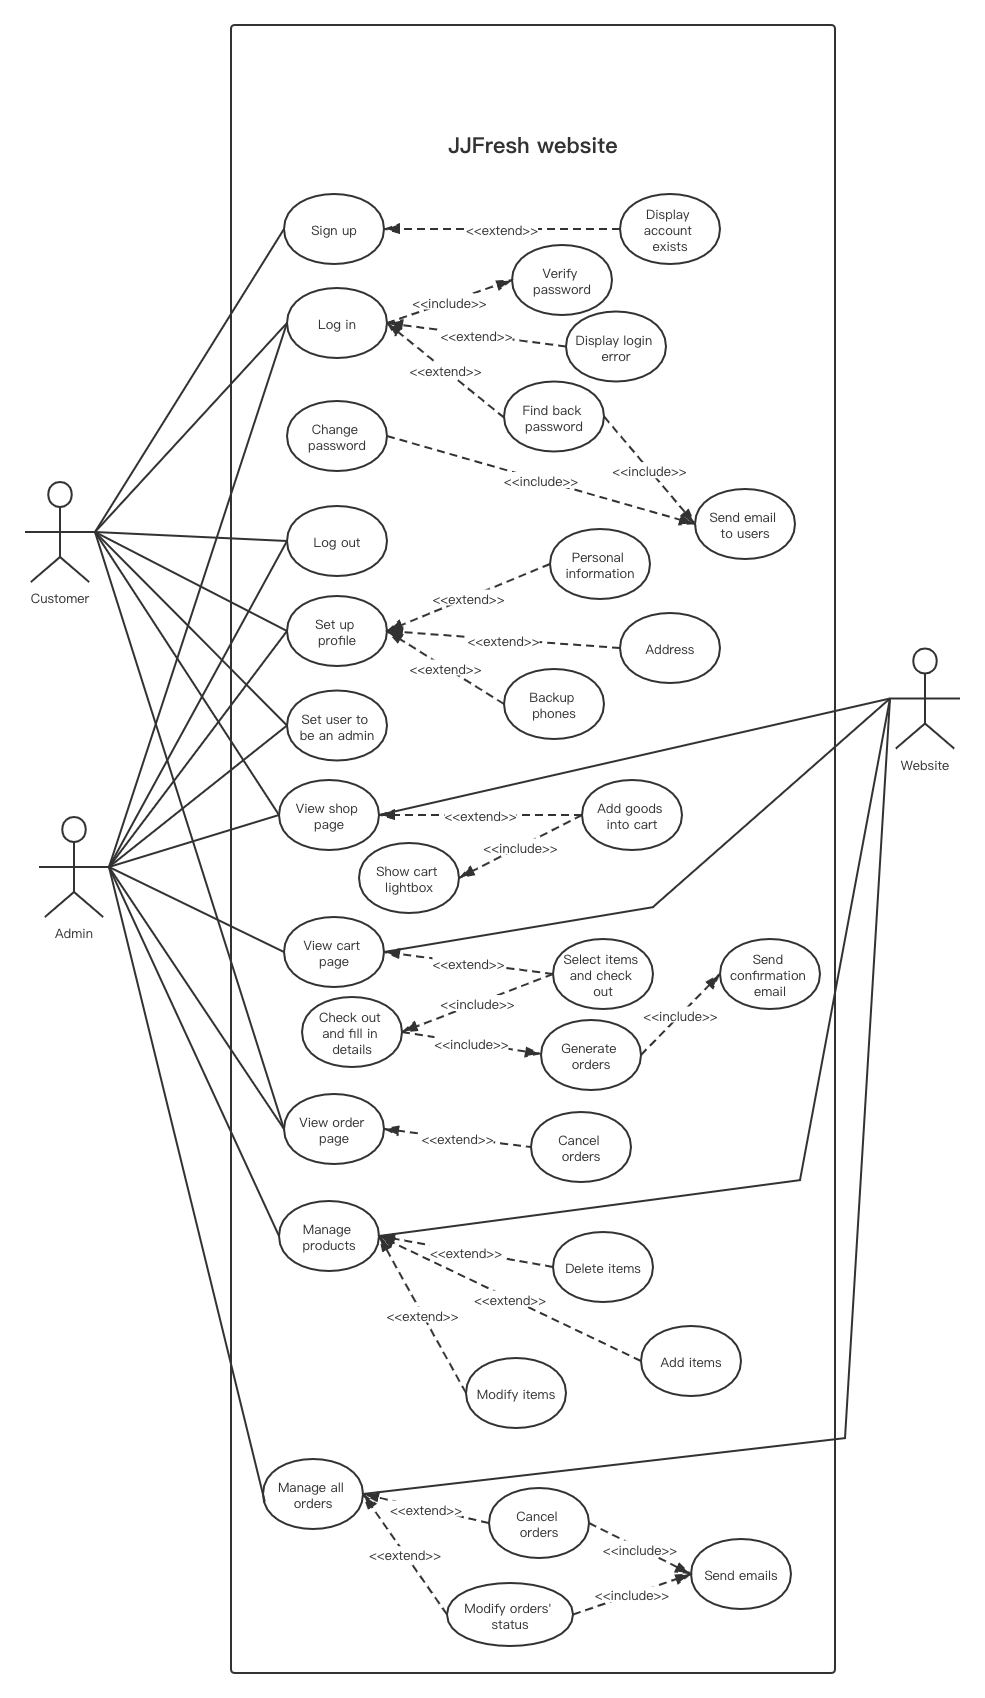
\includegraphics[width=0.5\textwidth]{Figures/useCaseDiagram.png}
\caption{Use Case Diagram}
\label{fig:useCaseDiagram}
\end{figure}


%%%%%%%%%%%%%%%%%%%%%%%%%%%%%%%%%%%%%%%%%%%%%%%%%%%%%%%%%%%%%%%%%%%%%%%%%%%%%%%%
\clearpage
\subsection{Risk Monitoring and Control}
\label{sub:riskMonitoringandControl2}
After the product owner simulated the use of this system, risk 3 occurred.

Team member Tian Yicun simulates Jess and James for order processing and merchandising, and team member Li Hongkang simulates multiple users for shopping. This risk was detected after users frequently placed orders and canceled orders for no reason.

Our team used pre-defined solutions to alleviate the risk to a certain extent. The specific operations are as follows. When the problem was discovered by Tian Yicun, Jess and James, she believed that the development team should add some functions as pre-defined. For example, when the same user frequently cancels orders withour reason, the number of orders he can cancel should be limited to one week. The development team currently sets the number of cancelled orders to 3. On the other hand, if the user orders a large number of vegetables Fruit, assuming that the total value exceeds 50 AUD, she should limit the time he can order, for instance, within 24 hours after placing the order, it can be cancelled.

After using the system with the above two functions added in the second simulation, they found that the risk occurrence rate was reduced, and the loss was within an estimated range. Therefore, the risk is reasonably controlled.

In addition, after discussion, we discovered a new risk, the specific definition and control are as follows:

\begin{tabularx}{0.95\linewidth}{%
  >{\raggedright\arraybackslash}p{1cm}%
  >{\raggedright\arraybackslash}p{1.2cm}%
  >{\raggedright\arraybackslash}p{2cm}%
  ll%
  >{\raggedright\arraybackslash}X}
  \toprule
  Risk ID & Risk Type & Description & Probability & Impact & Justification\\
  \midrule
  5
  & Business
  & Problems with suppliers, resulting in short supply of goods.
  & 40
  & 3
  & Because of the current impact of coronaviruses, the transportation and collection of vegetables and fruits are a serious problem. If the transportation time is too long, it will cause a shortage of supply. Besides many vegetables and fruits are susceptible to damage or rot due to bumps. If they do not pay attention to protection during transportation, the goods received by Jess and James may have quality problems,which will cause them to fail to complete the order on time and cause a certain economic loss.
  \\
  \bottomrule
  \\
  \label{Risk Monitor 1}
\end{tabularx}


\begin{table}
\begin{tabularx}{0.95\linewidth}{%
  >{\raggedright\arraybackslash}p{1cm}%
  >{\raggedright\arraybackslash}p{2cm}%
  >{\raggedright\arraybackslash}p{2cm}%
  >{\raggedright\arraybackslash}X%
  >{\raggedright\arraybackslash}p{2cm}%
  >{\raggedright\arraybackslash}p{2cm}}
  \toprule
  Risk ID & Trigger & Owner & Response & Response Strategy Type & Resources Required\\
  \midrule
  5
  & Suppliers are short of goods or have quality problems
  & Jess and James
  & Jess and James should find at least two suppliers. If one of them has problems, they can buy more from the other, so as to ensure the sufficient quantity of goods. In addition, they need to plan the purchase time reasonably so as not to be affected by the long transportation time.
  & Mitigate
  & Jess and James need to pay more attention to the situation of coronavirus and plan to purchase at least one week.
  \\
  \bottomrule
  \\
  \label{Risk Monitor 2}
\end{tabularx}
\end{table}
% \section{Project Status: Friday week 10}
% \subsection{Process Related Artefacts}
% \subsection{Product Related Artefacts}
% \subsection{Risk Monitoring and Control}